\section{Implementation of a QECC}
\label{sec:implementation}

In this section we are finally using the tools and methods presented in the last section to apply the quantum error correction (bit-flips) for the quantum Fourier transform.

\subsection{Implementing the quantum Fourier transform circuit}
\label{subsec:implementing-quantum-fourier-transform-circuit}

First and foremost it would make certainly sense to build the proposed QFT circuit and see if it actually works on a simulator and a real quantum device.
Recalling the basic concepts chapter we have already seen a generic circuit in figure~\ref{fig:qft-generic-circuit} that can be rebuilt using Qiskit.
The controlled \texttt{R}-gate is a rotation around the Z-axis which can be realized in \texttt{Qiskit} using a controlled \texttt{U1} gate~\cite{ControlledU1Gate}.

Before using \emph{Qiskit} and building the circuit we need to set up the code by listing the needed imports in appendix~\ref{subsec:qft-circuit-qiskit-necessary-imports} for \emph{Python}.
Afterwards we can follow the circuit in figure~\ref{fig:qft-generic-circuit} and implement it iteratively for any size in Qiskit as seen in appendix~\ref{subsec:qft-function}.
That allows us creating an arbitrarily big circuit.
One example circuit graph for 4 input qubits is created and shown in figure~\ref{fig:qft-4-qubit-circuit}.
Note that the circuit is mirrored vertically compared to the reference circuit, as Qiskit is ordering the qubits differently compared to most resources~\cite{QiskitGettingStarted}.

\begin{figure}[H]
    \centering
    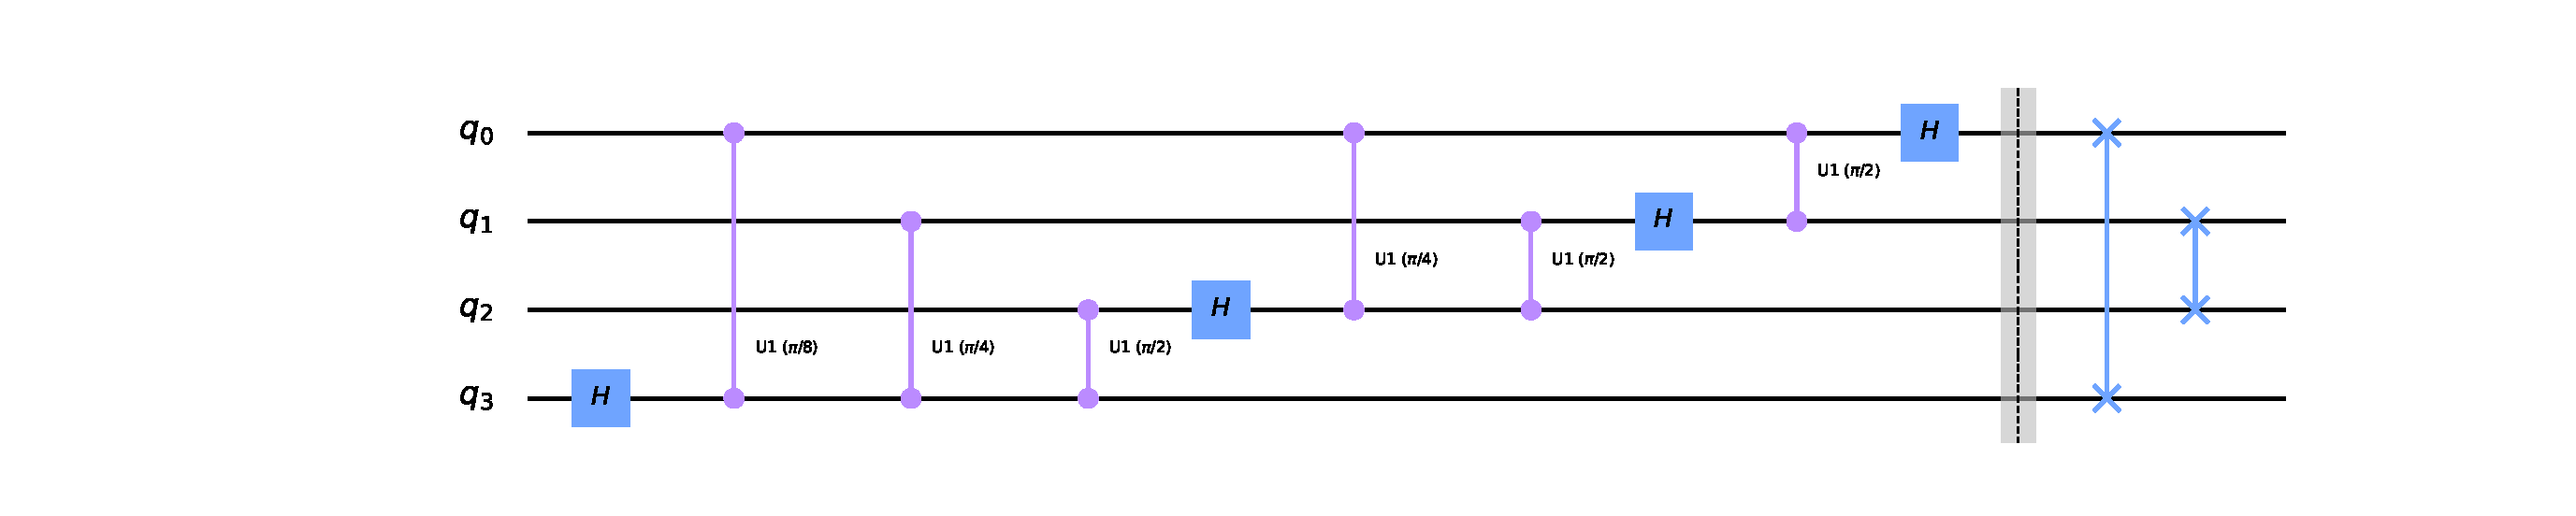
\includegraphics[width=\textwidth]{res/qft-4-qubits-circuit.pdf}
    \caption{Qiskit 4-qubit QFT circuit graph}
    \label{fig:qft-4-qubit-circuit}
\end{figure}

To get the inverse of that circuit \emph{Qiskit} offers the method \texttt{inverse()} which can be applied on any \texttt{QuantumCircuit}.
It is applied in the function displayed in appendix~\ref{subsec:inverse-qft-function} and delivers together with the non-inversed QFT the circuit depicted in figure~\ref{fig:qft-4-qubit-circuit-with-inverse}.

\begin{figure}[H]
    \centering
    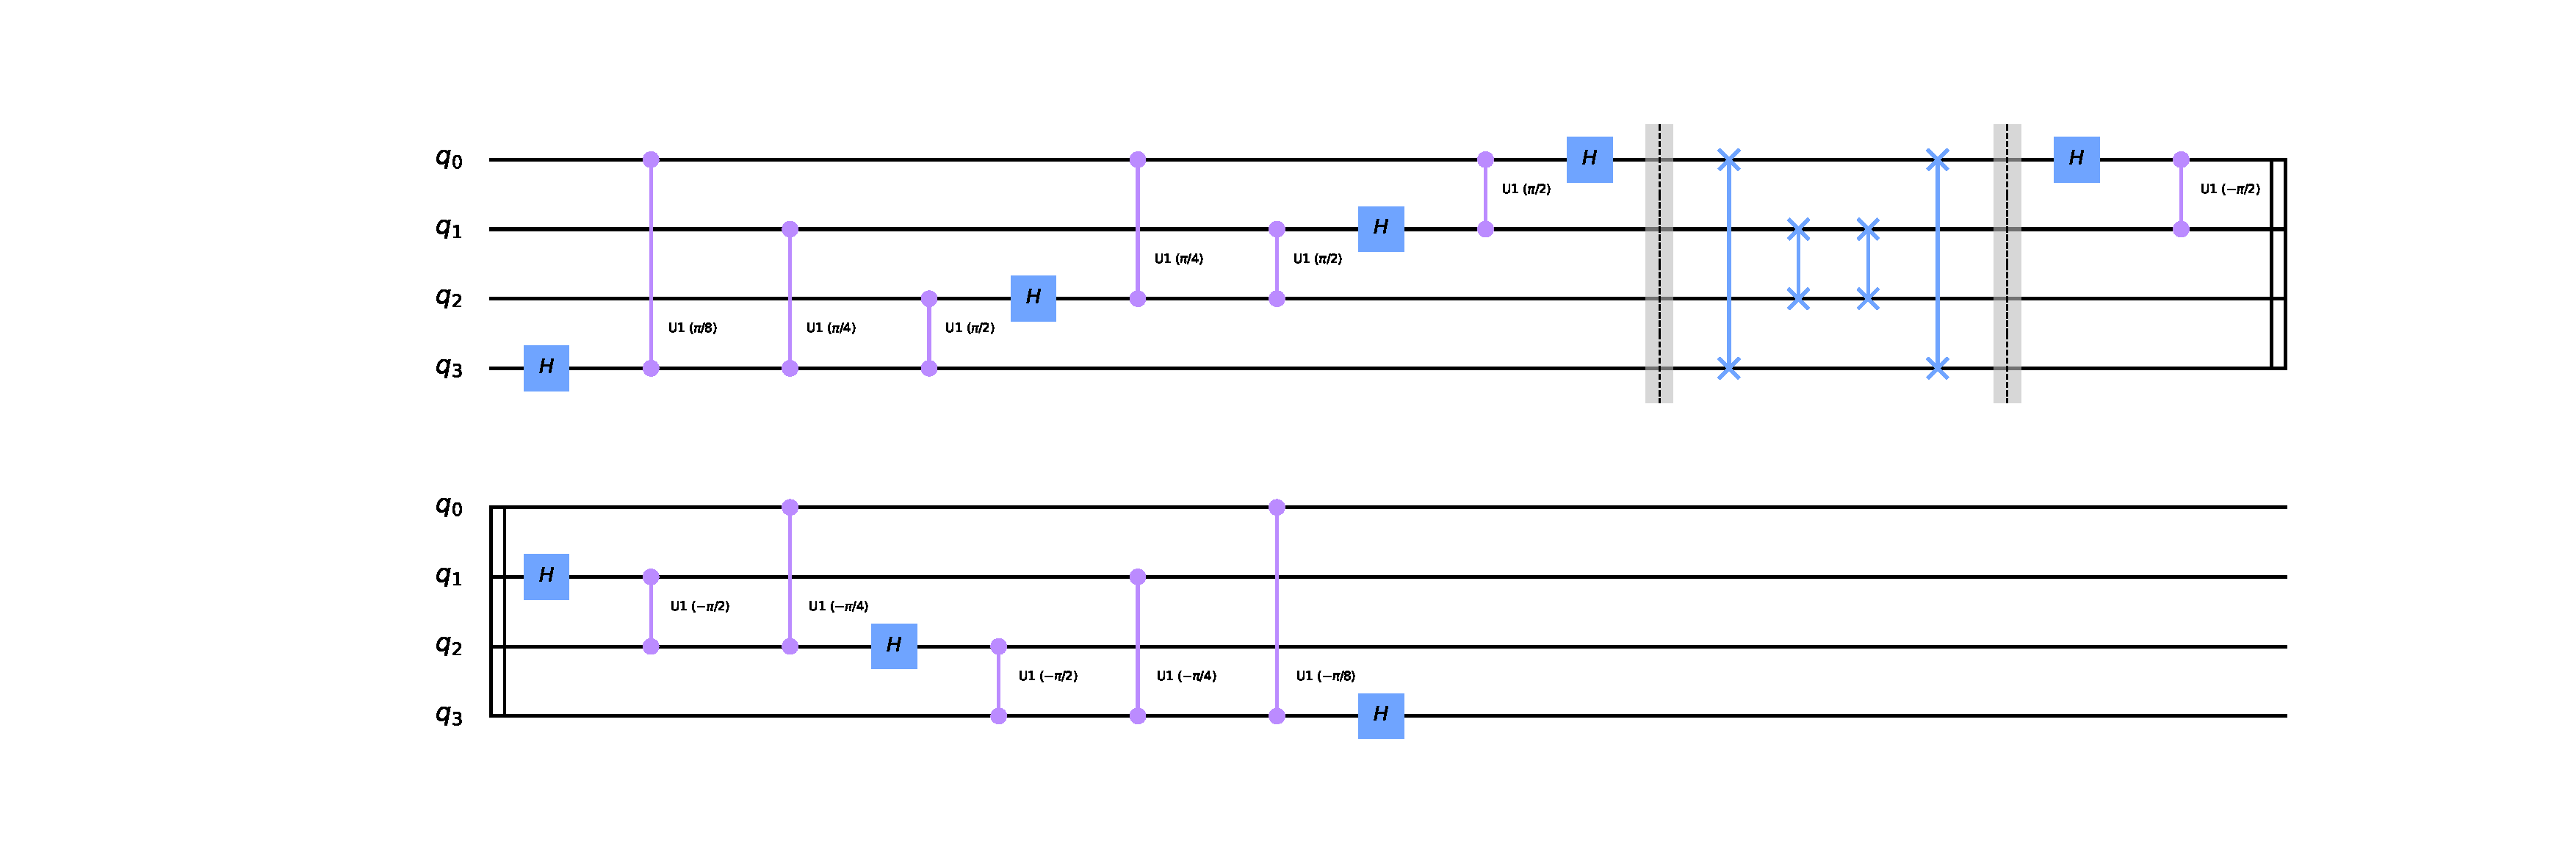
\includegraphics[width=\textwidth]{res/qft-4-qubits-circuit-with-inverse.pdf}
    \caption{Qiskit 4-qubit QFT + inverse QFT circuit}
    \label{fig:qft-4-qubit-circuit-with-inverse}
\end{figure}

The last step to have a fully functional circuit, is to encode a number to the qubits that serve as the input.
A method in appendix~\ref{subsec:encoding-decoding-number-in-circuit} is written that encodes a number to a binary string and later to another quantum circuit that is scaled to fit the amount of needed bits to represent the passed number.
For example the decimal integer number 12 is encoded to the binary string \texttt{1100} and therefore needs the circuit to have 4 input qubits.
Additionally, the same code in the appendix shows a function to measure the qubits to classical bits at the end of the circuit to get the circuits result as binary string again.
That result should ideally match the input when no error occurs.

The full circuit for the encoded number \(6\) (\texttt{110}) is shown in figure~\ref{fig:full-qft-3-qubit-circuit}.

\begin{figure}[H]
    \centering
    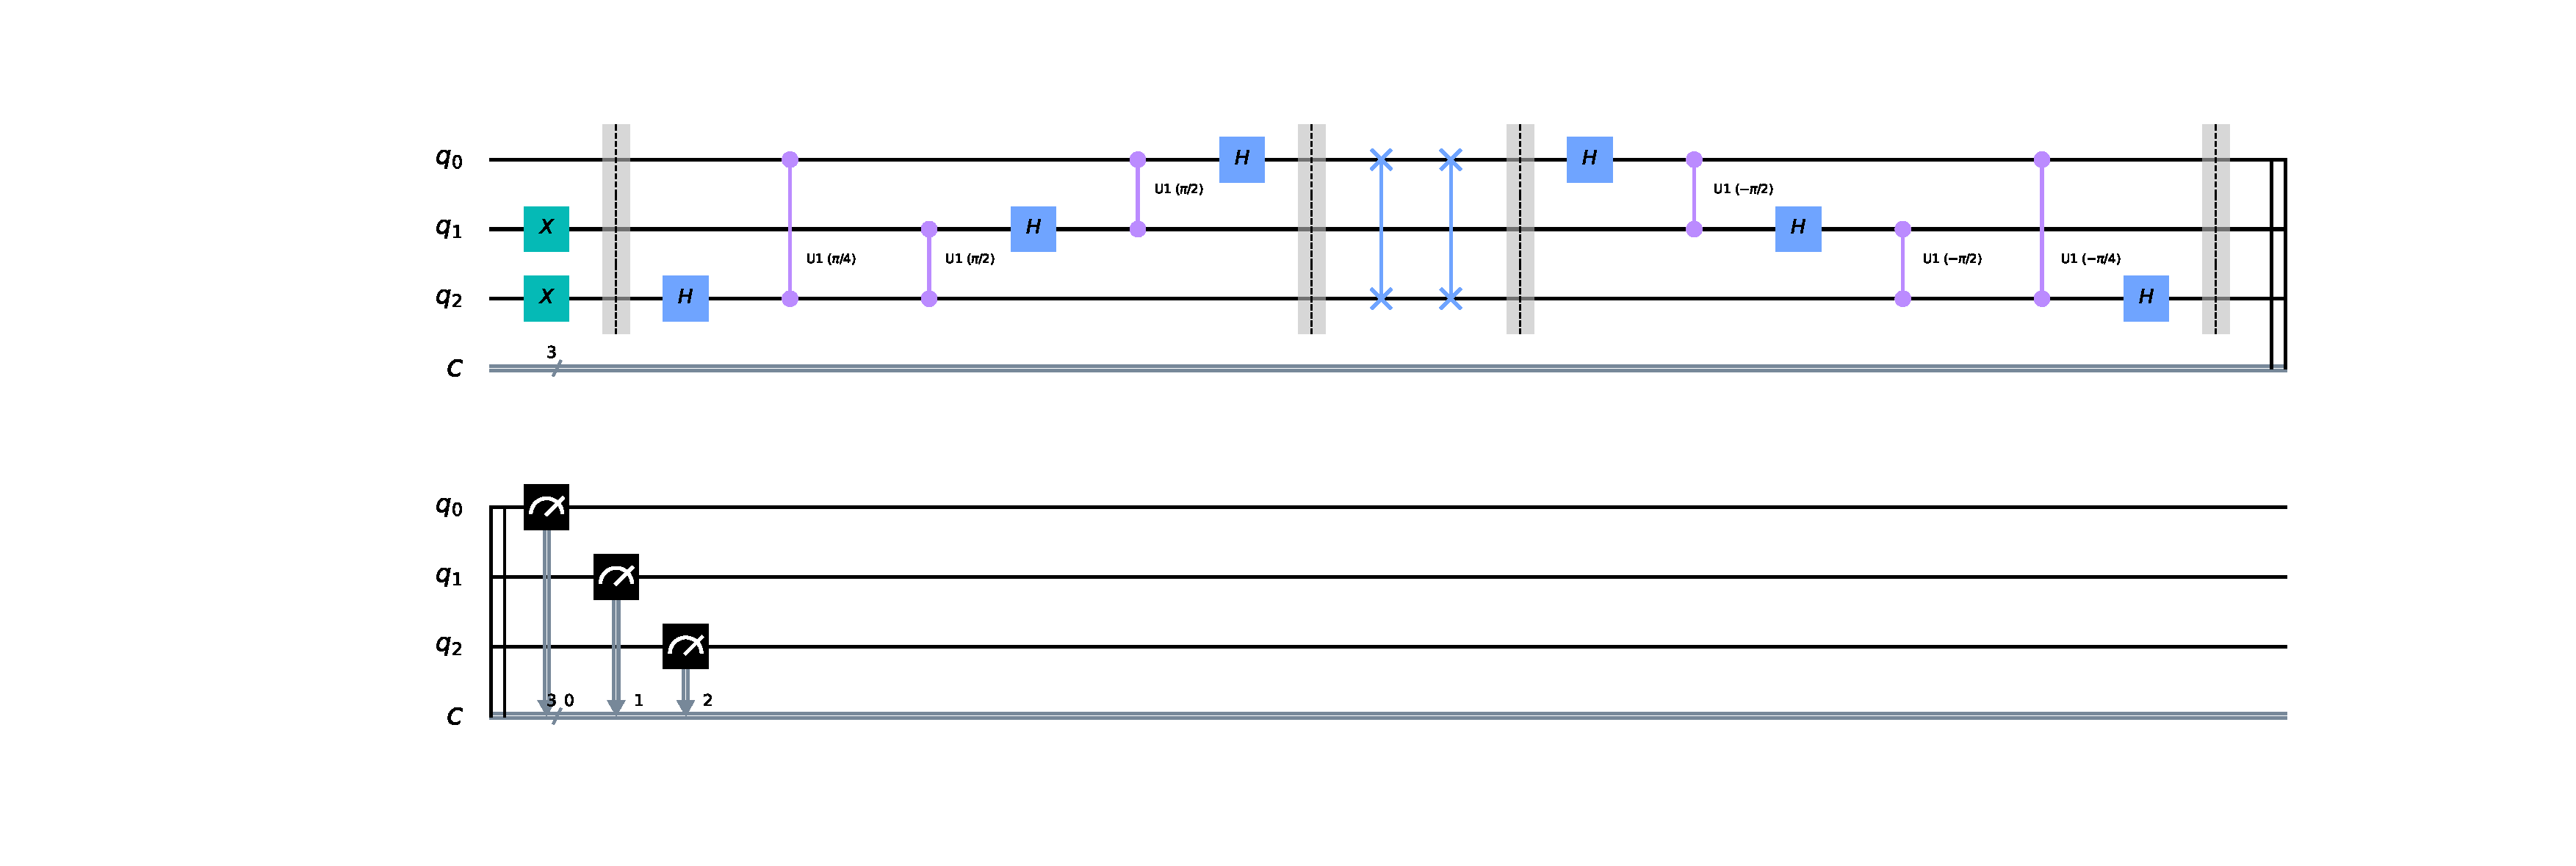
\includegraphics[width=\textwidth]{res/full-qft-3-qubit-circuit.pdf}
    \caption{Qiskit 3-qubit circuit used in this paper}
    \label{fig:full-qft-3-qubit-circuit}
\end{figure}

For the sake of completeness, the source code for generating the above image is listed in Annex~\ref{subsec:generating-full-qft-circuit}.

\paragraph{Testing}

Now that we have the circuit we should be able to test it using the Qiskit simulator and a real quantum device.
The simulator testing is done using the code from~\ref{subsec:testing-circuit-simulator-no-noise} from which figure~\ref{fig:test-histogram} is created.
The histogram is showing \(1024\) simulated results from the circuit.
Since we have not configured the simulator to simulate noise the result is the same (\texttt{110}) for all shots as expected.

\begin{figure}[H]
    \centering
    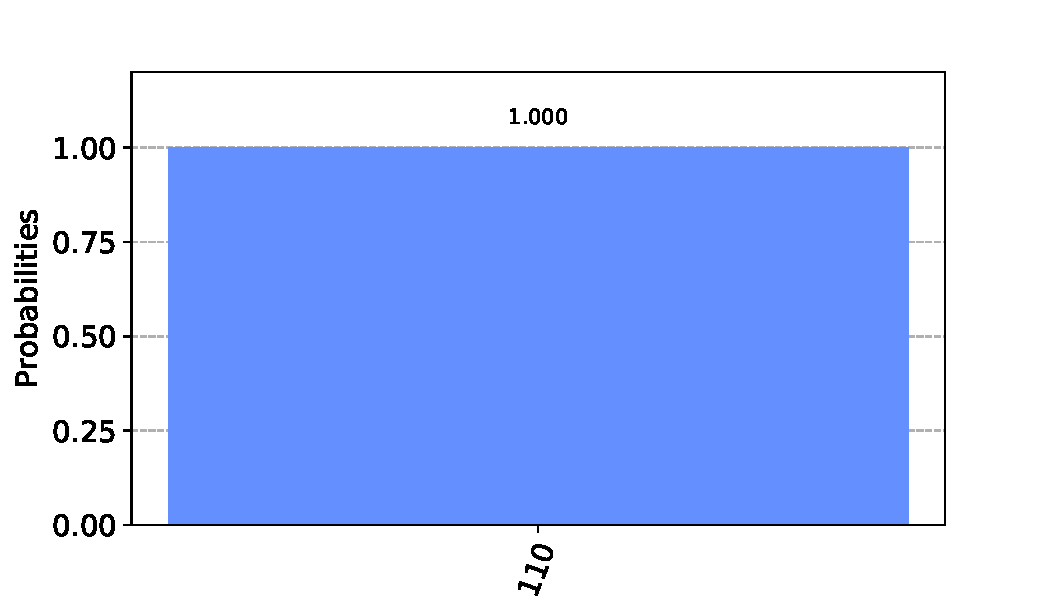
\includegraphics[width=0.7\textwidth]{res/test-histogram.pdf}
    \caption{Simulator result without noise for the full proposed QFT circuit with 3 qubits}
    \label{fig:test-histogram}
\end{figure}

We are able to simulate noise using the \texttt{noise\_model} parameter of Qiskits \texttt{execute} function.
\citeA{QiskitErrorCorrection} showed a function to create a noise model from which we derived the one listed in appendix~\ref{subsec:noise-model-function}.
It anticipated two parameters:
\begin{enumerate}
    \item The probability \(p_{error_{measurement}}\) that the measurement leads to a bit-flip
    \item The probability \(p_{error_{gate}}\) to replace the state of a qubit with a random state
\end{enumerate}

Another way of creating a noise model is by automatically generating one from the properties of a real quantum device using the \texttt{NoiseModel.from\_backend()} method~\cite{QiskitDocsNoise}.
In the first test we'll settle with manually specifying the probabilities to both \(5 \%\).
Later a noise model is generated from a real quantum backend followed by executing the circuit on the real device.

The code for generating the simulated results as shown in the histogram in figure~\ref{fig:test-histogram-with-noise} is listed in appendix~\ref{subsec:testing-circuit-simulator-noise}.
It is evident that there is indeed noise as we do no more measure the correct result \texttt{110} with \(100 \%\) probability.

\begin{figure}[H]
    \centering
    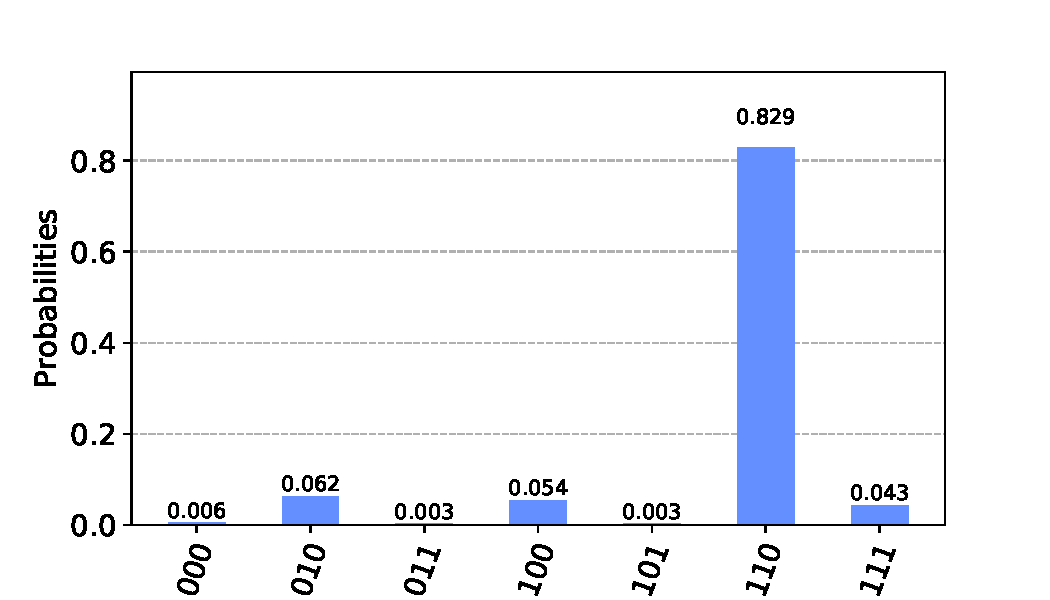
\includegraphics[width=0.7\textwidth]{res/test-histogram-with-noise.pdf}
    \caption{Simulator result \textbf{with} noise for the full proposed QFT circuit with 3 qubits}
    \label{fig:test-histogram-with-noise}
\end{figure}

Now we try generating a noise model from a real quantum backend.
The code to do that is as always placed in the appendix~\ref{subsec:testing-circuit-generated-noise-model}.
It is choosing the least busy quantum device.
In the case of the resulting figure~\ref{fig:test-histogram-generated-noise-model} it has chosen a backend called \texttt{ibmqx2}.
If we compare it with the previous histogram, we find that it has produced a noise model that is not as noisy as the \(5 \%\) gate and measurement errors we selected earlier.

\begin{figure}[H]
    \centering
    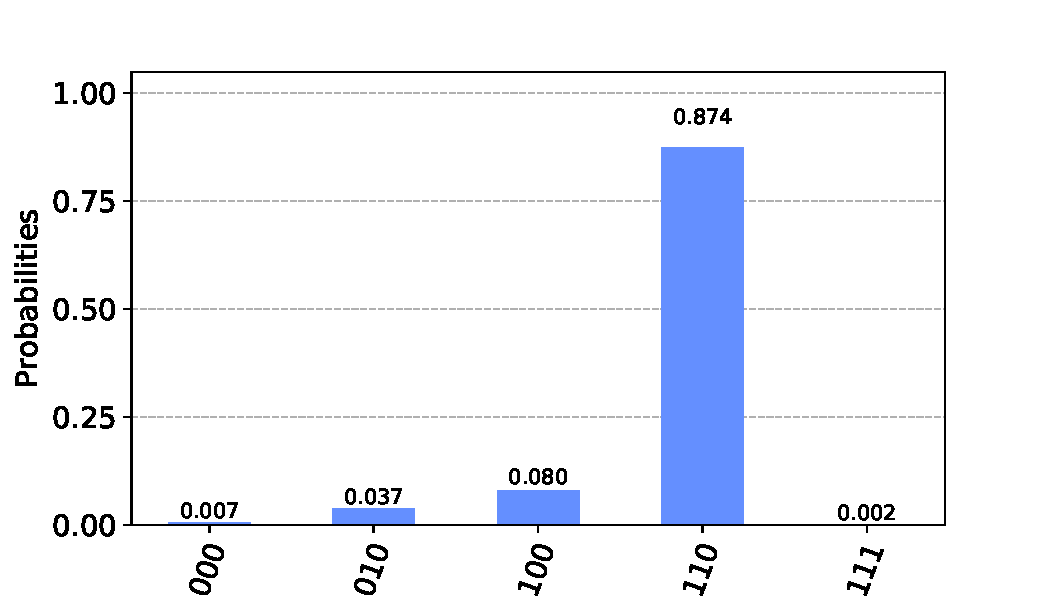
\includegraphics[width=0.7\textwidth]{res/test-histogram-generated-noise-model.pdf}
    \caption{Real quantum device result for the full proposed QFT circuit with 3 qubits}
    \label{fig:test-histogram-generated-noise-model}
\end{figure}

The resulting histogram for the test with a real quantum device, which can be generated using the code from appendix~\ref{subsec:testing-circuit-real-device}, is depicted in figure~\ref{fig:test-histogram-real-device}.
Another result the code is outputting is the quantum backend name on which the circuit has been executed.
In this case the name is \texttt{ibmqx2}.
That happens to be the same that Qiskit has generated a noise model for.
Comparing it to the actual results we see a huge difference as the actual noise seems to be greater.

\begin{figure}[H]
    \centering
    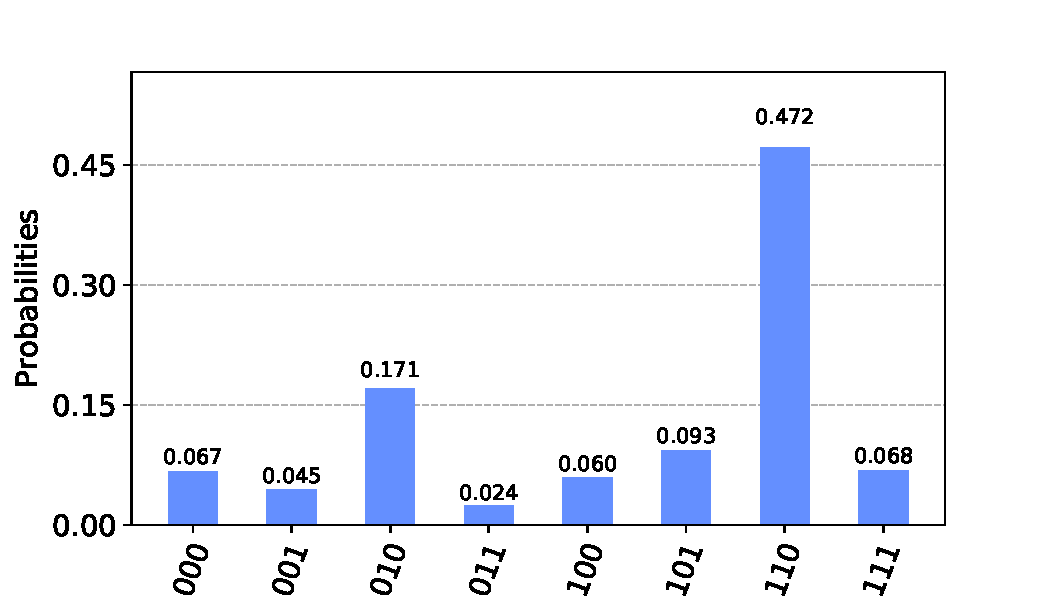
\includegraphics[width=0.7\textwidth]{res/test-histogram-real-quantum-device.pdf}
    \caption{Real quantum device result for the full proposed QFT circuit with 3 qubits}
    \label{fig:test-histogram-real-device}
\end{figure}

\subsection{QFT circuit changes for error-correction}
\label{subsec:qft-circuit-error-correction}

We now are applying some changes in order to correct bit-flip errors in the circuit.
A good result would be a better looking histogram than the ones listed above.

To keep the circuit relatively small we will stick with the 3-qubit QFT circuit and repeat it 3 times.
That means we have to stack the previously shown circuit vertically and add some ancillary qubits.
The functions in appendix~\ref{subsec:modified-qft-circuit-functions} are rewritten versions of the previously shown ones that allow passing a parameter specifying a quantum circuit object to apply the gates on as well a vertical \texttt{offset} to apply them in the passed circuit.
This is done to have the code reusable, small and still comprehensible.

Additionally those functions are used in another function \texttt{prepare\_rc\_qec\_qft\_circuit} which can be seen in appendix~\ref{subsec:circuit-building-code}.
It is building the whole circuit for a specified input number and repetition count.
An example for 2 input qubits and 3 repetitions is displayed in figure~\ref{fig:example-error-correction-circuit} but it really can be any size.
As one can see we need 4 ancillary qubits for correcting bit flips at the end.
For 3 input qubits and 3 repetitions it would be 6 ancillary qubits.
Thus we conclude a formula for determining the needed ancillary qubit count \(c_{ancilla}\) for a given input qubit size \(c_{qubits}\) and repetitions \(c_{rep}\):

\[
    c_{ancilla}(c_{qubits}, c_{rep}) = (c_{rep} - 1) * c_{qubits}
\]

The ancilla qubits are needed per qubit in the QFT circuit.
Since we repeat the QFT circuit multiple times we need more ancilla qubits.
For 3 input qubits and 3 repetitions we need two ancilla qubits per qubit in a single QFT circuit suming up to 6 since they compare for example all three first qubits of all repetitions as seen in figure~\ref{fig:ancillary-qubit-count}.

\begin{figure}
    \centering
    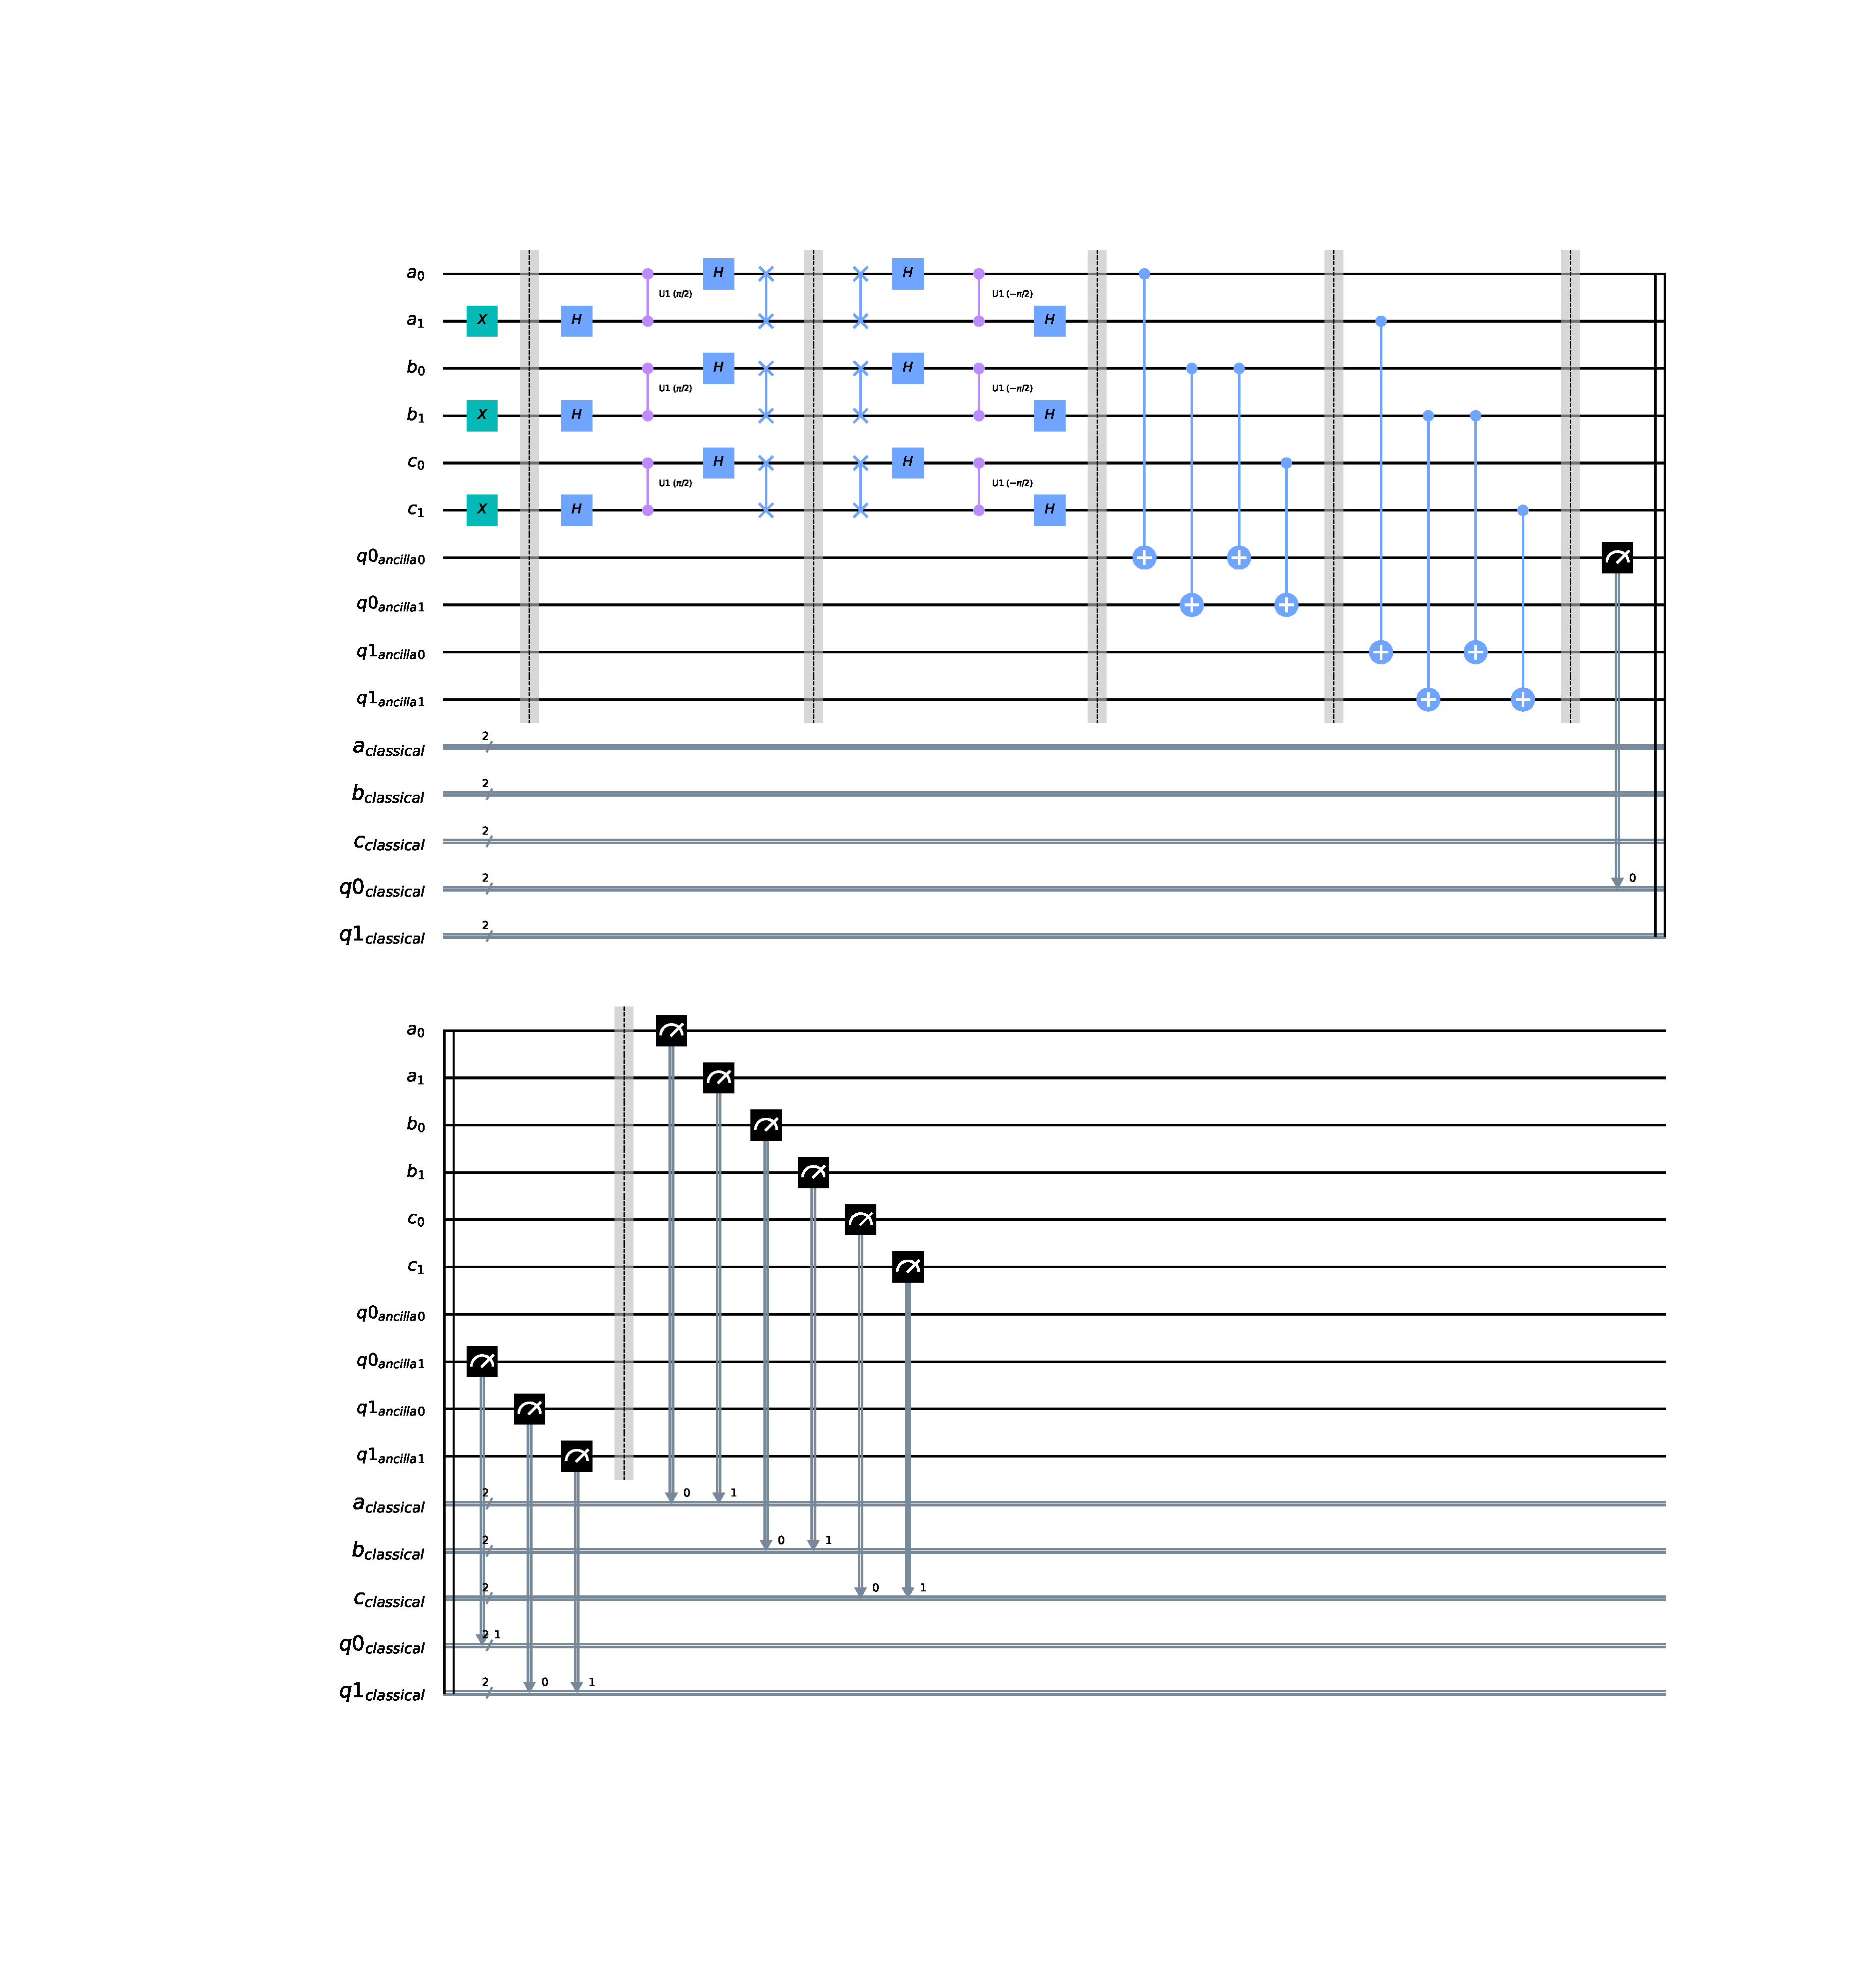
\includegraphics[width=\textwidth]{res/example-error-correction-circuit.pdf}
    \caption{Error corrected QFT circuit with 2 qubits input and 3 repetitions}
    \label{fig:example-error-correction-circuit}
\end{figure}

\begin{figure}[H]
    \centering
    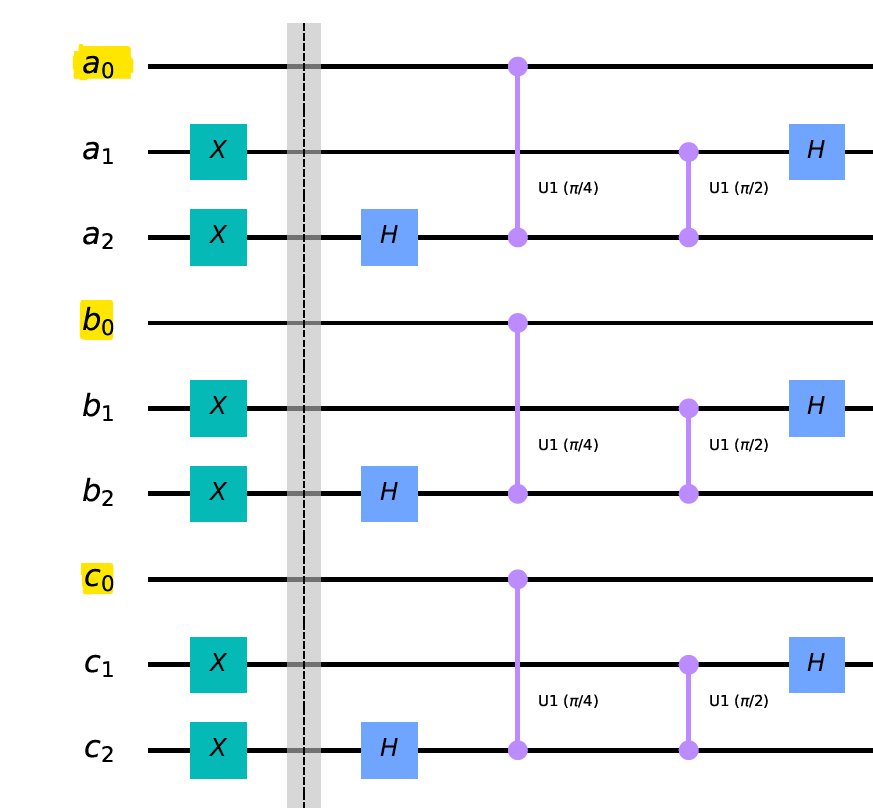
\includegraphics[width=0.5\textwidth]{res/highlighted-qubits.png}
    \caption{Snippet from the error correcting circuit with 3 input qubits and 3 repetitions. The first qubits of every repetition that are essentially duplicates are highlighted. For those we introduce ancillary qubits in order to compare them at the end.}
    \label{fig:ancillary-qubit-count}
\end{figure}

The last code snipped can be looked up in appendix~\ref{subsec:appendix-decoding-result-circuit} and is decoding a resulting bit string from the circuit.
That means correcting the error when the ancillary bits indicate one.
As an example we decode the possible result string \texttt{10 01 00 010 110 010}.
The first three bit strings \texttt{10}, \texttt{01} and \texttt{00} are the measured results from the ancillary qubits.
Those indicate whether an error happened.
The concrete meaning is summarized in the following table.

\begin{center}
    \begin{tabular}{ r c l }
        \texttt{00} & \(\Rightarrow\) & No error happened \\
        \texttt{01} & \(\Rightarrow\) & Error happened in the first QFT register (Qubit \(a_0, a_1 or a_2\)) \\
        \texttt{10} & \(\Rightarrow\) & Error happened in the last QFT register (Qubit \(c_0, c_1 or c_2\)) \\
        \texttt{11} & \(\Rightarrow\) & Error happened in the middle QFT register (Qubit \(b_0, b_1 or b_2\))
    \end{tabular}
\end{center}

Additionally to that, the position of the ancillary bit strings indicate the exact qubit the error occurred on.
So in the example the error \texttt{10} occurred on the third, \texttt{01} on the second and \texttt{00} (No error) on the first qubit of the specified register.

\begin{center}
    \begin{tabular}{ r c l }
        \texttt{10} & \(\Rightarrow\) & Error at \(c_2\) \\
        \texttt{01} & \(\Rightarrow\) & Error at \(a_1\) \\
        \texttt{00} & \(\Rightarrow\) & No error at \(a_0, b_0 or c_0\) \\
    \end{tabular}
\end{center}

Since we are trying to correct bit-flips we can just flip the resulting bits in the remaining 3 QFT result strings \texttt{010} (Register \(c\)), \texttt{110} (Register \(b\)) and \texttt{010} (Register \(a\)).
According to the ancillary qubits we have to flip \(c_2\) and \(a_1\) which results in the three corrected strings \texttt{110} (Register \(c\)), \texttt{110} (Register \(b\)) and \texttt{000} (Register \(a\)).
When merging that three strings we get \texttt{110} as \textbf{decoded} result.
In summary that is exactly what the decoding function does.

\paragraph{Testing}

As quick reminder: We now have functions to generate a error correcting circuit via repetition of the initial QFT circuit we proposed.
Additionally, we have introduced the resulting bit string format which we will get from the Qiskit simulator as well as the real quantum backends.

This section aims at testing a 3 input qubit, 3 repetitions circuit with the encoded number 6 using the simulator as well as real quantum devices.
In the first step we will use the Simulator with manually chosen and generated noise models, followed by some real quantum backends.

Utilizing the code displayed in appendix~\ref{subsec:code-histogram-results} we are able to generate histograms showing the decoded results for multiple execution shots of the quantum circuit.
The histograms are plotted on the same result set but with different error correcting techniques applied:
\begin{itemize}
    \item \textbf{No error correction}: No error correction is applied on the result set and all the results from the individual QFT circuit repetitions are taken into account.
    \item \textbf{Only merging results}: The results from the individual QFT circuits are merged, but the ancillary bit result is not taken into account.
    \item \textbf{Error correction}: The results from the individual QFT circuits are first error corrected using the ancillary bit results and then merged.
    \item \textbf{Only merge results without error}: Only results from the individual QFT circuits are merged that have not been flagged as wrong by the ancillary bit results.
\end{itemize}

Figure~\ref{fig:test-histogram-qec-results-noise-model} is visualizing the results when using the simulator with a noise model with both probability values set to \(5 \%\).

\begin{figure}[H]
    \centering
    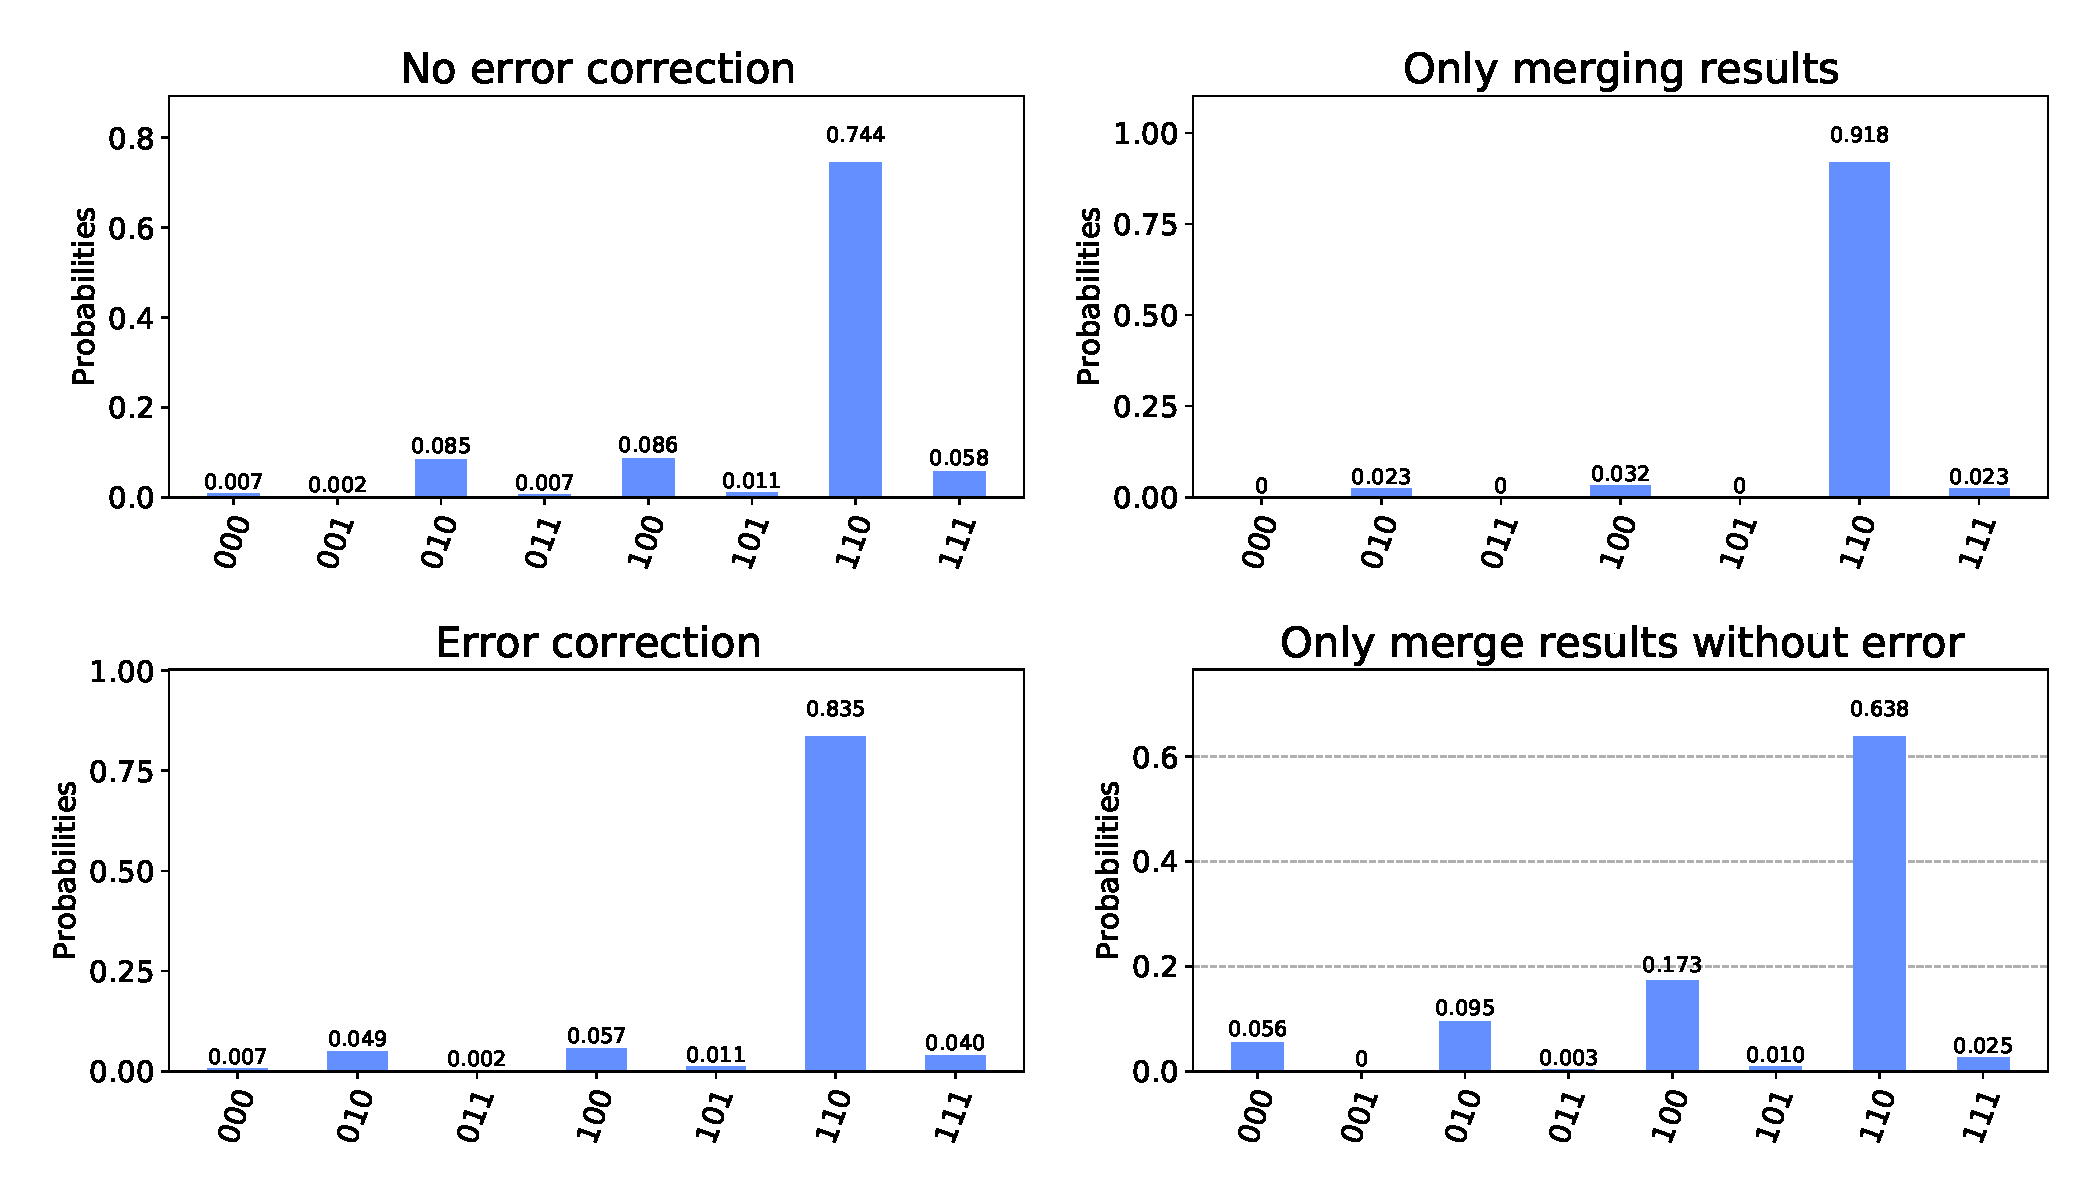
\includegraphics[width=0.95\textwidth]{res/test-histogram-qec-results-noise-model.pdf}
    \caption{Result distributions of 1024 shots of the proposed error correcting circuit.}
    \label{fig:test-histogram-qec-results-noise-model}
\end{figure}

The histograms show that the error correction is indeed working by increasing the correct result ratio from \(0.744 \%\) to \(0.835 \%\).
Interestingly only merging the results without error correction seems to work even better.

When generating a noise model using Qiskit from the backend \texttt{ibmq\_16\_melbourne} we get the results from figure~\ref{fig:test-histogram-qec-results-noise-model-generated}.

\begin{figure}[H]
    \centering
    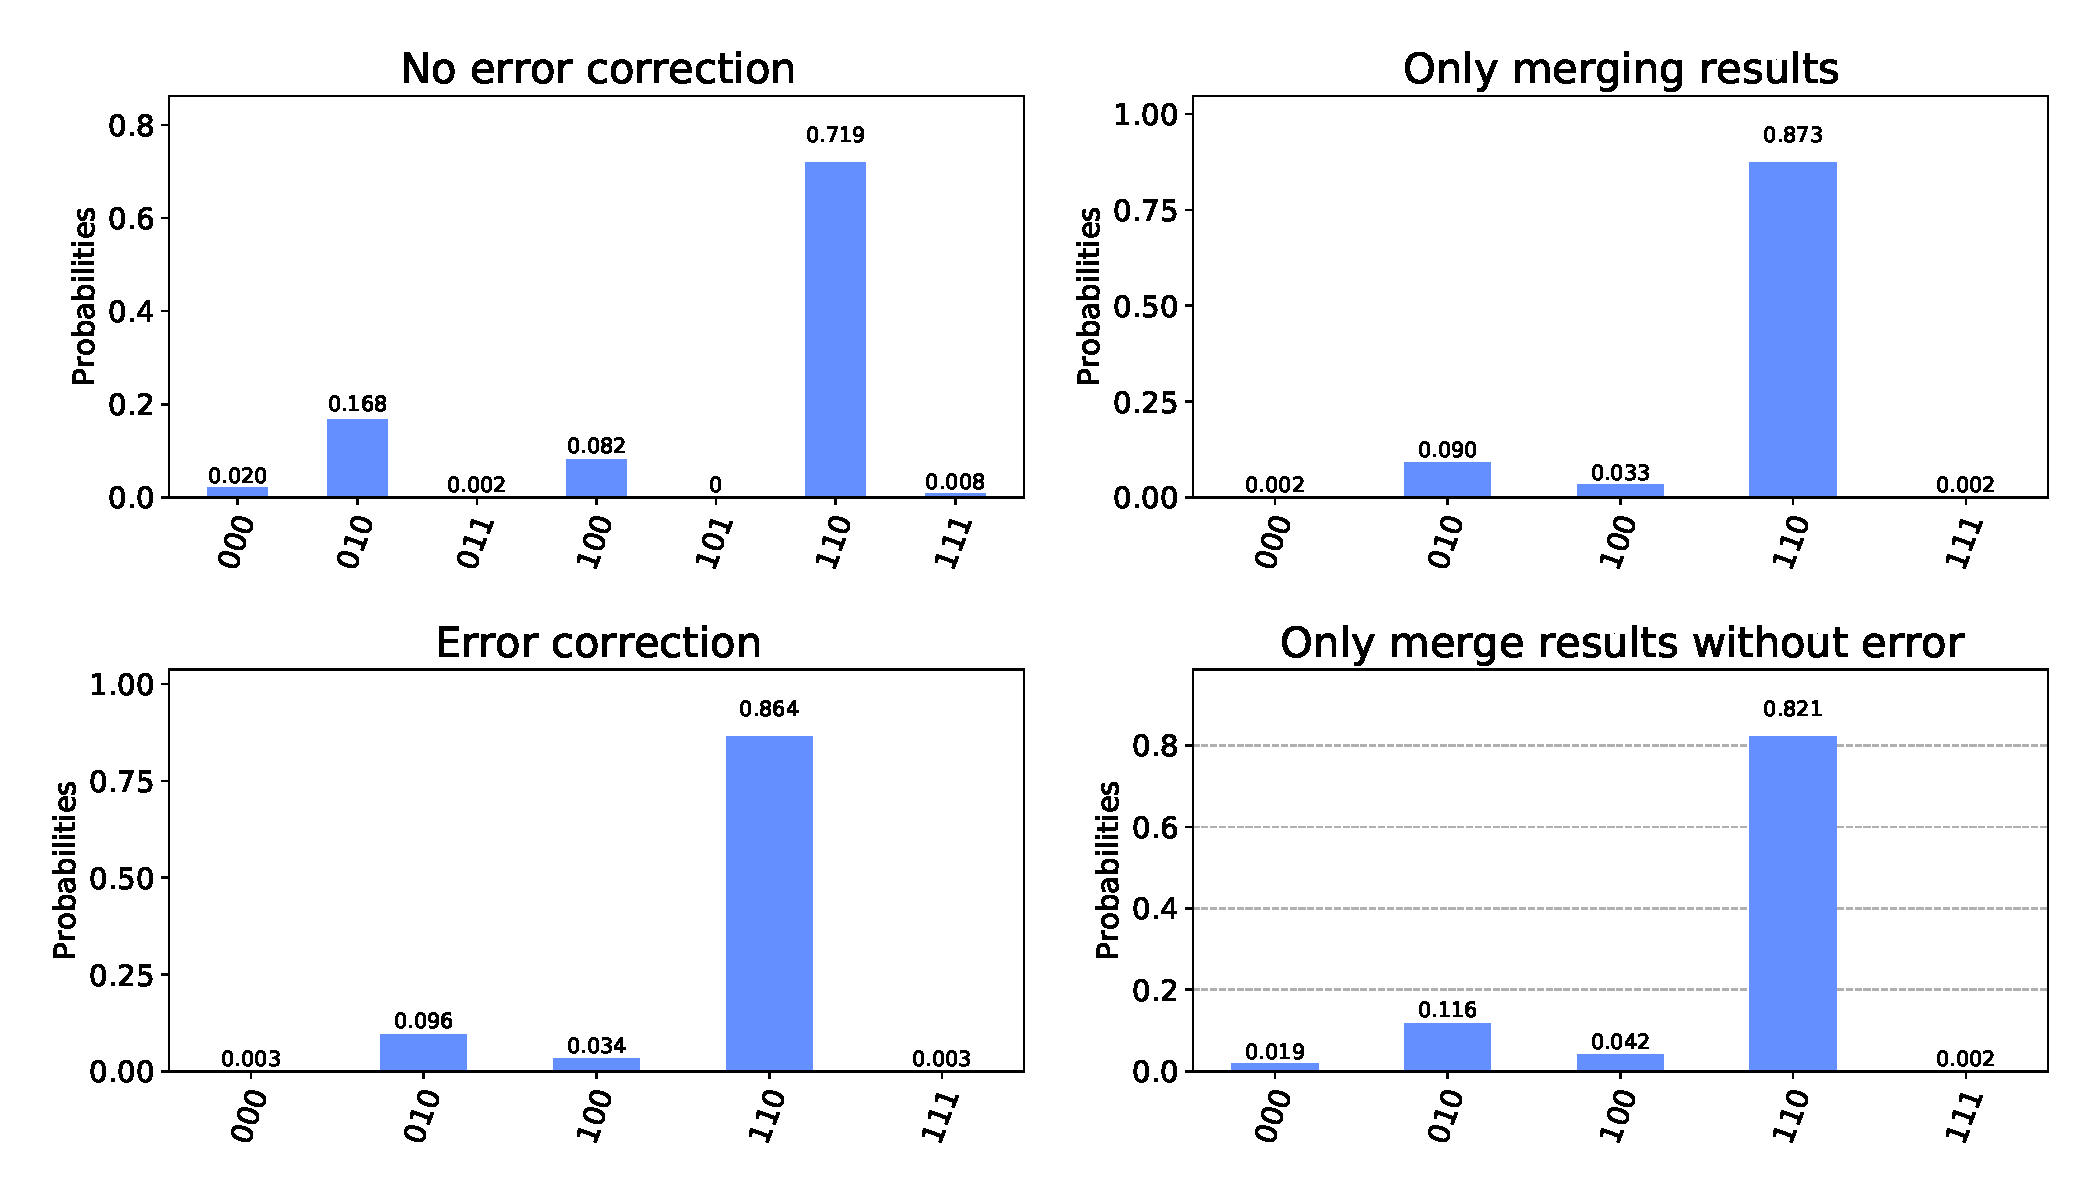
\includegraphics[width=\textwidth]{res/test-histogram-qec-results-noise-model-generated.pdf}
    \caption{Result distributions of 1024 shots of the proposed error correcting circuit using a generated noise model from the backend \texttt{ibmq\_16\_melbourne}.}
    \label{fig:test-histogram-qec-results-noise-model-generated}
\end{figure}

Again the results show an improvement when using error correction but with less difference between the "Error correction" and "Only merging results" plots compared to the manually configured noise model.

Running on the real quantum backend \texttt{ibmq\_16\_melbourne} we get the results displayed in the below plots of figure~\ref{fig:test-histogram-qec-results-noise-model-melbourne}.
Unfortunately that backend seems to be too noisy and results in mostly random results.

\begin{figure}[H]
    \centering
    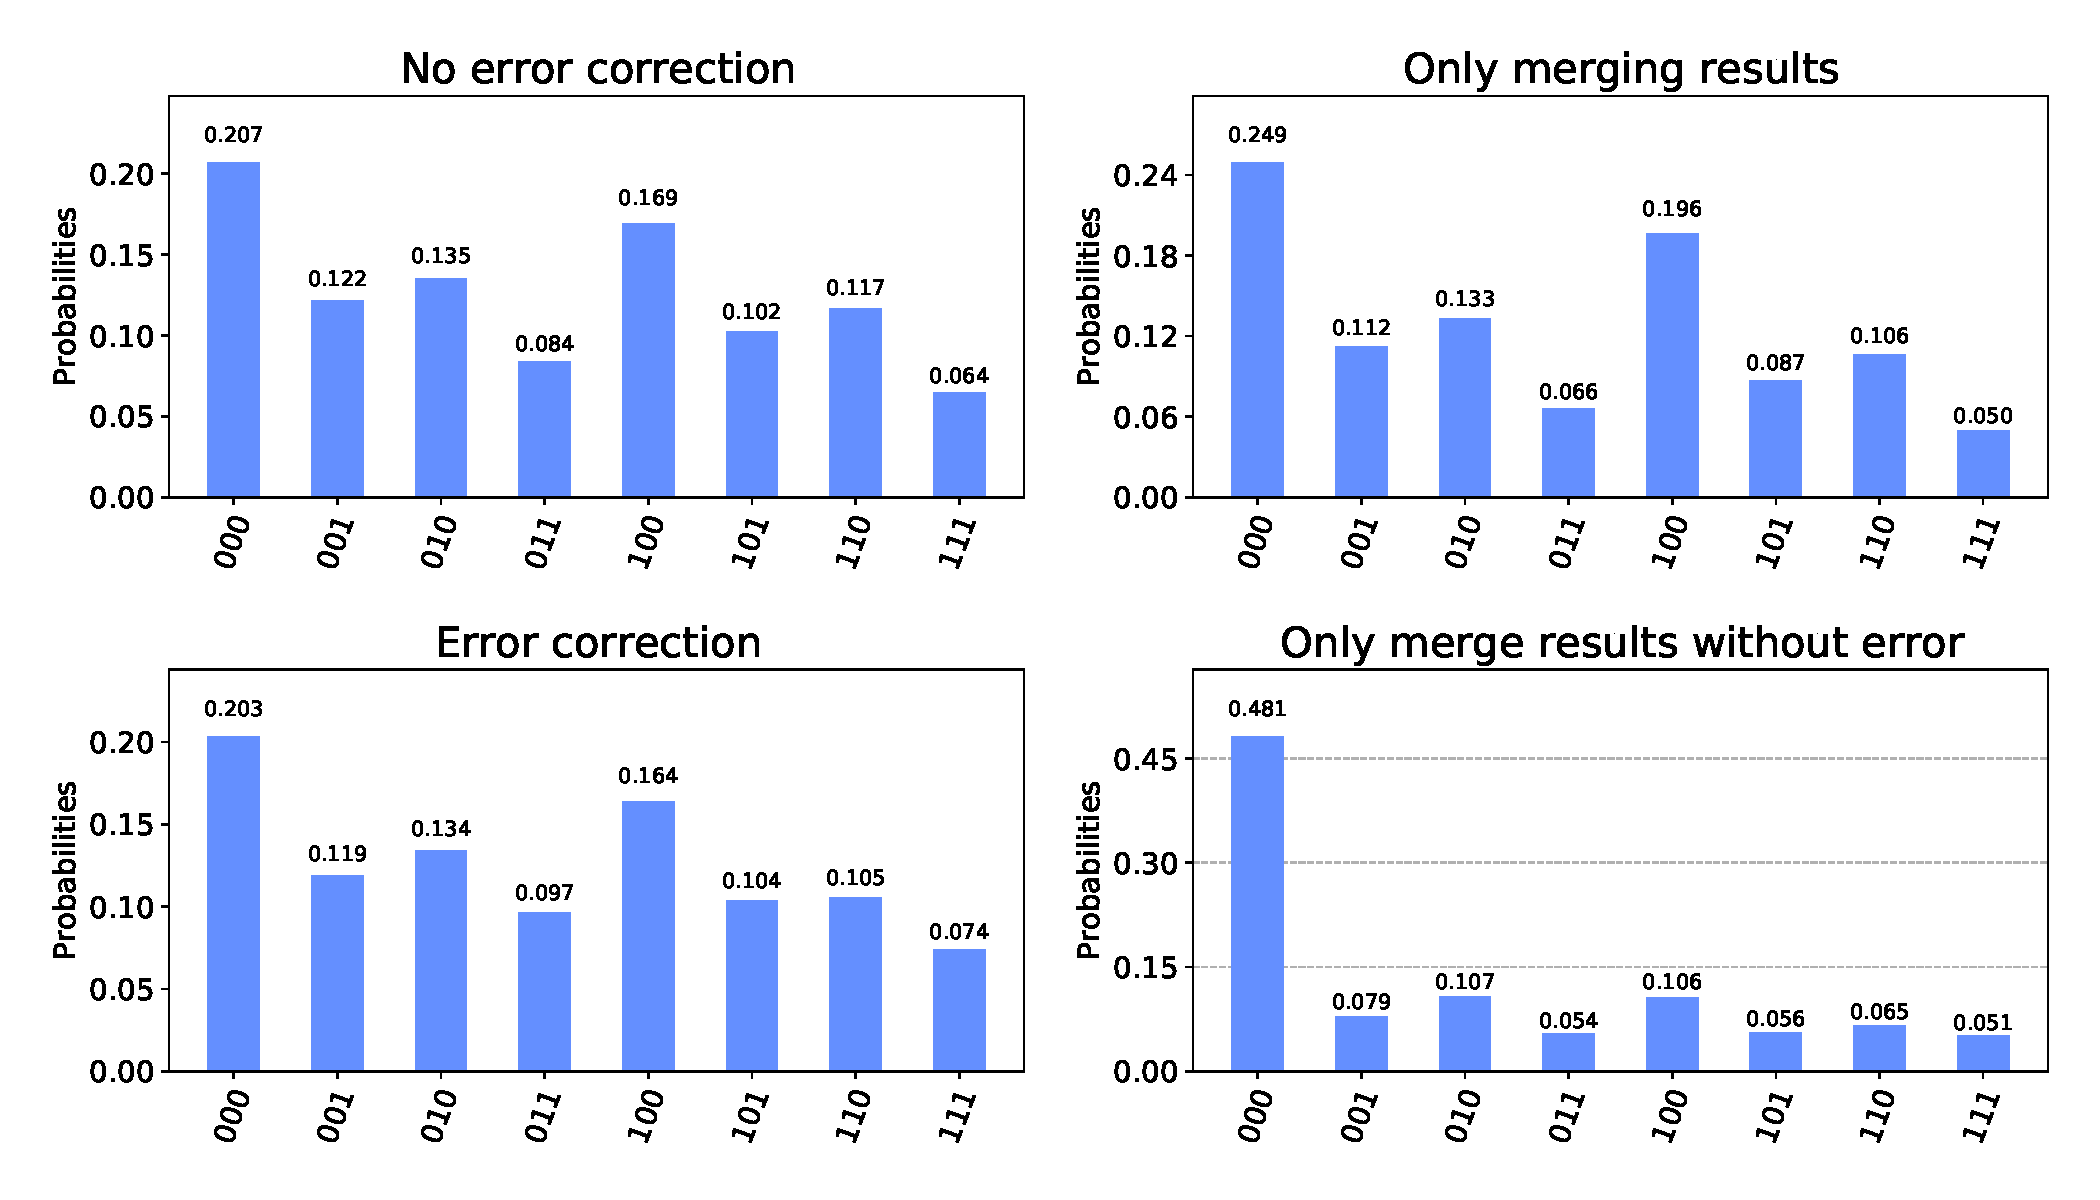
\includegraphics[width=0.95\textwidth]{res/test-histogram-qec-results-melbourne.pdf}
    \caption{Result distributions of 1024 shots of the proposed error correcting circuit using the backend \texttt{ibmq\_16\_melbourne}.}
    \label{fig:test-histogram-qec-results-noise-model-melbourne}
\end{figure}

Additionally the circuit has been executed on two more sophisticated quantum devices "Paris" (27 qubits) and "Johannesburg" (20 qubits) leading to the results displayed in figure~\ref{fig:test-histogram-qec-results-paris} and~\ref{fig:test-histogram-qec-results-johannesburg}~\cite{IBMQAvailableSystems}.

\begin{figure}[H]
    \centering
    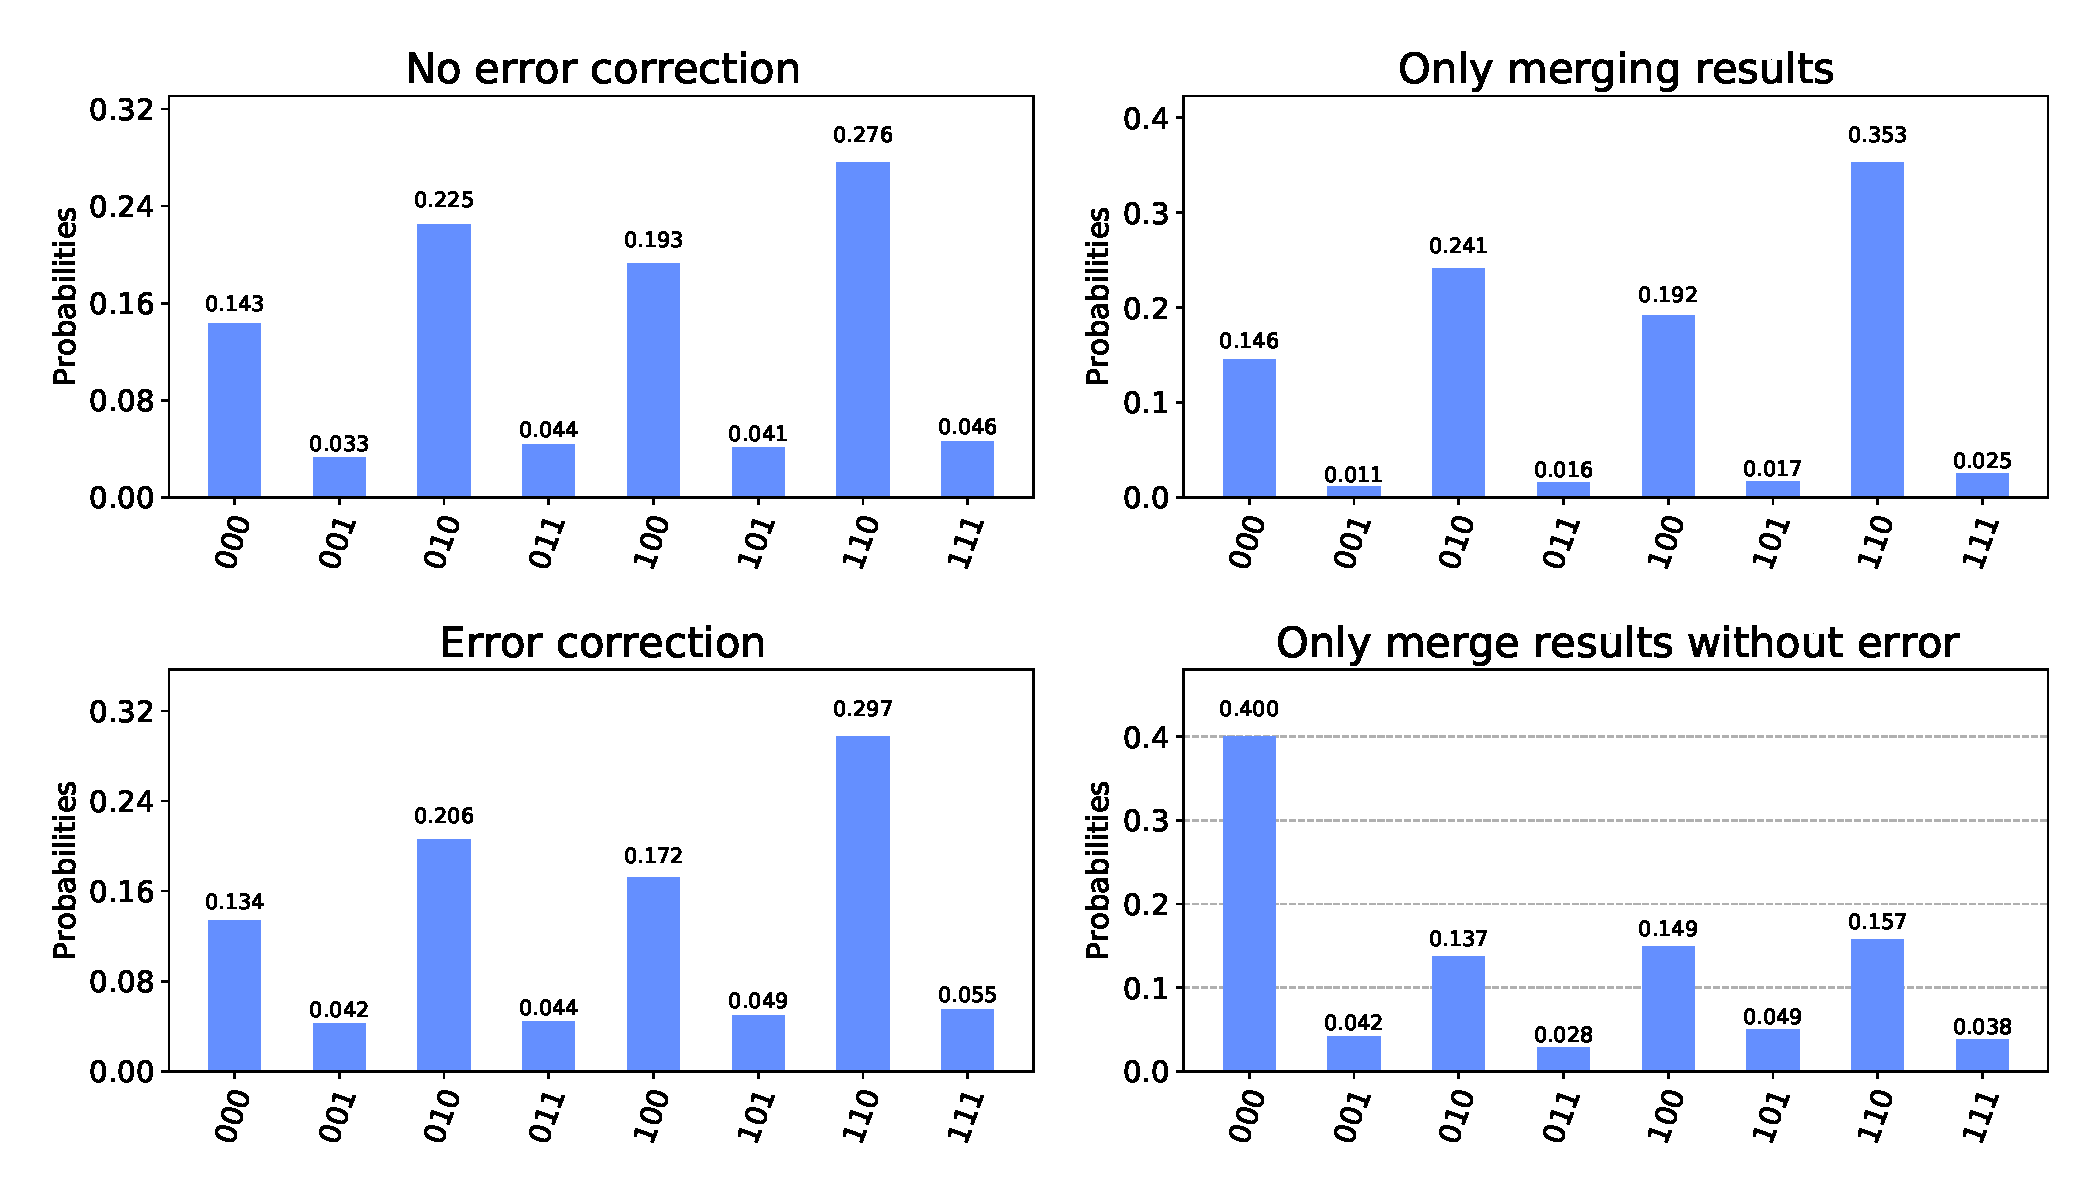
\includegraphics[width=0.95\textwidth]{res/test-histogram-qec-results-paris.pdf}
    \caption{Result distributions of the proposed error correcting circuit using the backend "Paris" with 27 qubits.}
    \label{fig:test-histogram-qec-results-paris}
\end{figure}

\begin{figure}[H]
    \centering
    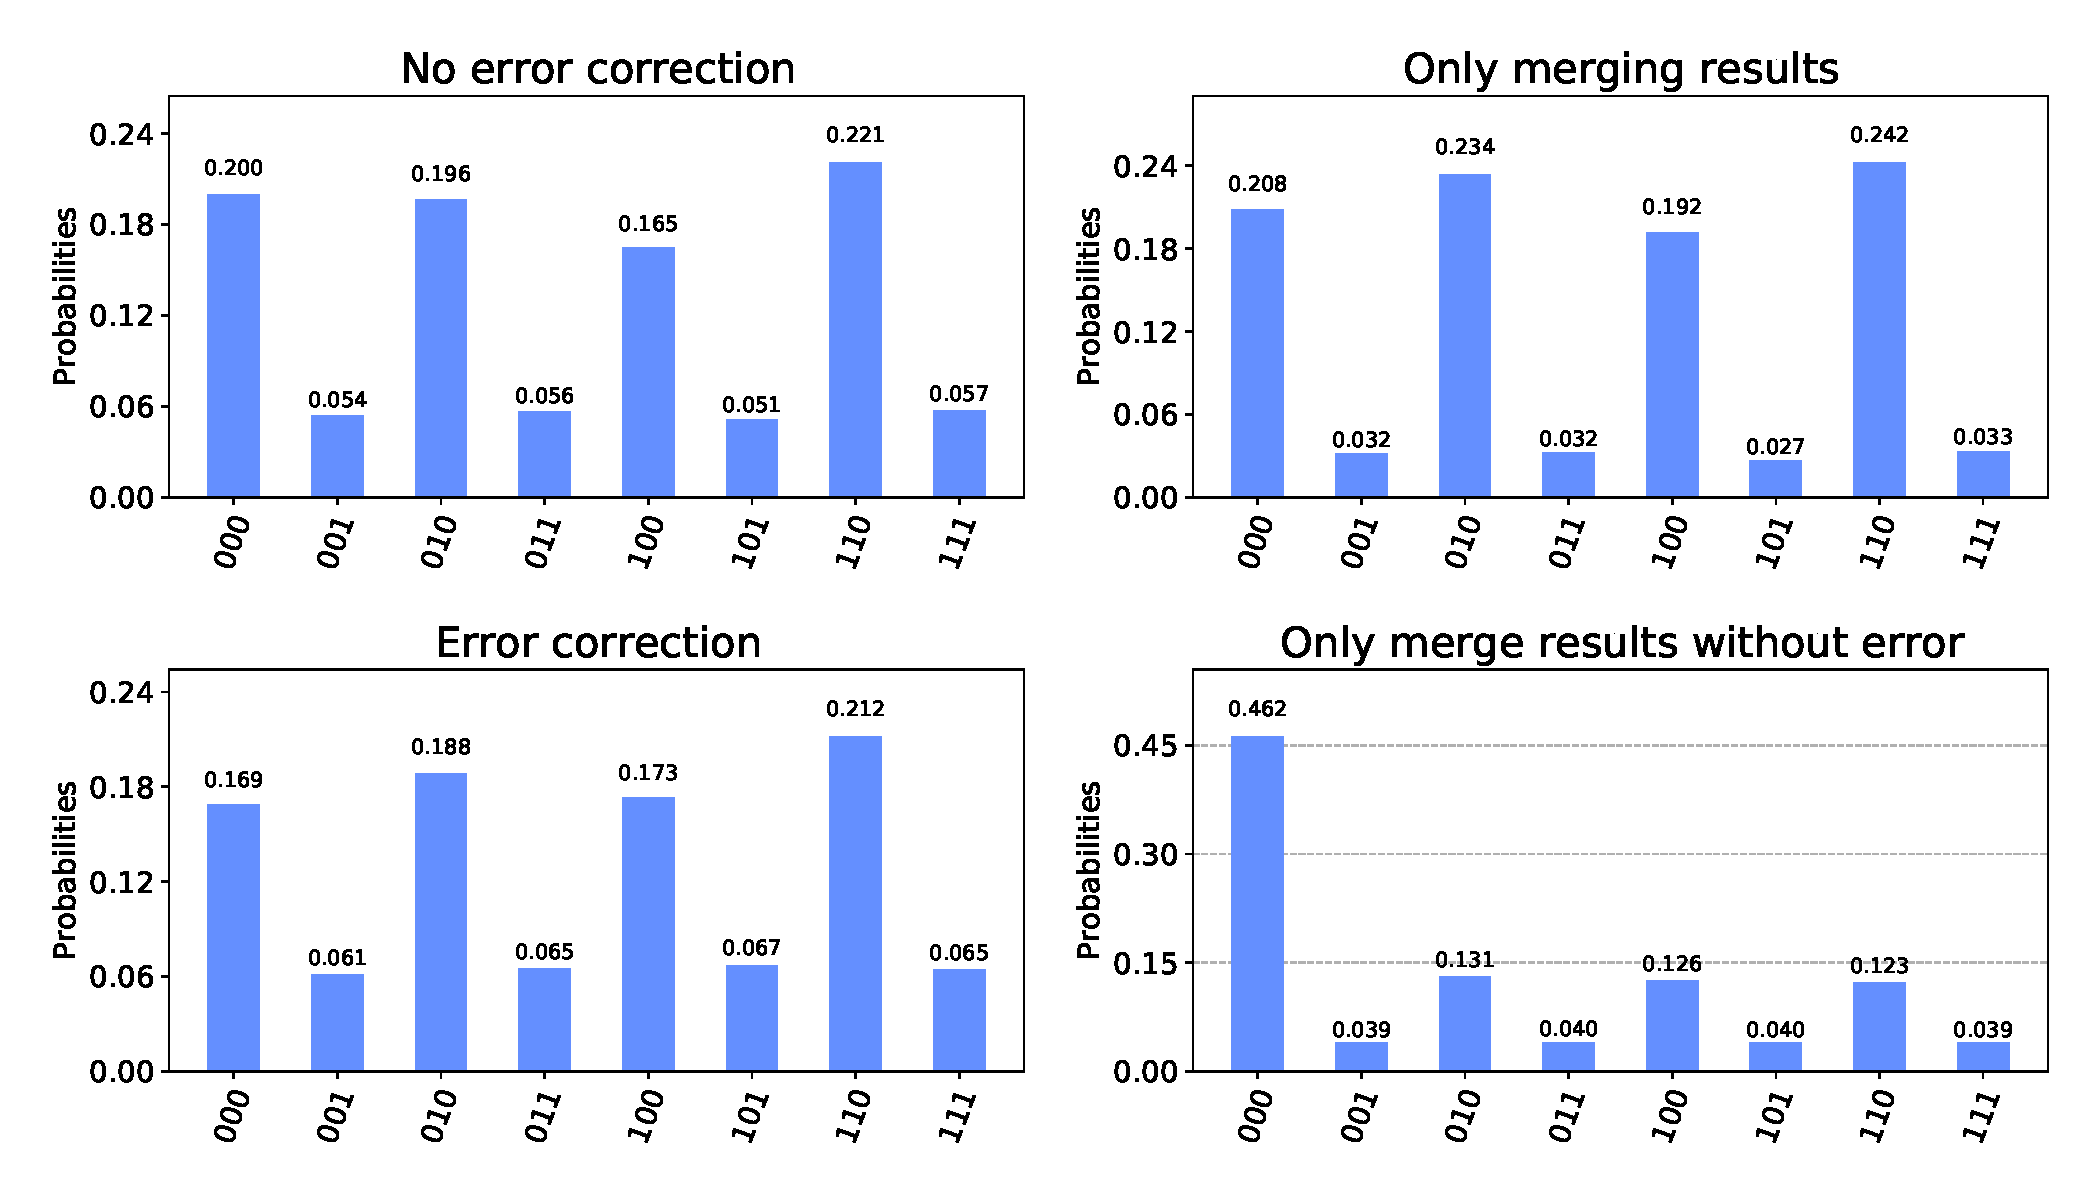
\includegraphics[width=\textwidth]{res/test-histogram-qec-results-johannesburg.pdf}
    \caption{Result distributions of the proposed error correcting circuit using the backend "Johannesburg" with 20 qubits.}
    \label{fig:test-histogram-qec-results-johannesburg}
\end{figure}

While there is still a lot of noise observable - at least for the proposed circuit - we can definitely see that error correction is working.
Especially on "Paris" where "Only merging results" provides a jump from \(0.276 \%\) to \(0.353 \%\).
"Paris" is also the only one of the tested real quantum backends where "Error corrections" does show an improvement compared to "No error correction".
